In the previous chapter we have assumed that the state was fully measurable, i.e. the matrix $C=I$. This hypotesis in general does not hold for real world applications and so in order to design a \textit{cooperative control system} we first need to \textbf{estimate the state} $x_i$ of each agent. \\
This is the reason that leads us to design a \textbf{design a device} which provides an \textbf{estimate} $\hat{x}_i$ of the state $x_i$ \textbf{for each agent} such that 
\begin{equation}
    \lim_{t \to \infty} \hat{x}(t) = x(t)
\end{equation}

\section{Cooperative observer design for a single agent}
The only information can be shared among the agents is the \textbf{local output estimation error} which is defined as
\begin{equation}
    \tilde{y}_i = y_i - \hat{y}_i = y_i - C \hat{x}_i 
\end{equation}
For the design of the \textbf{local observer} is important also another quantity that is the \textbf{neighbourhood output estimation error} which is defined as: 
{\large
    \begin{equation}
        \xi_i = \sum_{j=1}^N {a_{ij} (\tilde{y}_j - \tilde{y}_i) + g_i(\tilde{y}_0 - \tilde{y}_i)}
    \end{equation}
}
Finally for a single agent in a cooperative context, the \textbf{cooperative observer} is by 
\begin{equation} \label{eq: coop_OBSV}
    \dot{\hat{x}}_i = A \hat{x}_i + B u_i - cF\xi_i
\end{equation}
This cooperative protocol leads to a \textbf{completely distributed observer} in the sense that is based only on: 
\begin{itemize}
    \item The \textbf{local output estimation error} $\tilde{y}_i$
    \item The \textbf{estimation error} of the neighbours which is expressed by the succint number $\xi_i$
\end{itemize} 

\section{Global estimation error and global observer}
We can pack together the equations for the local cooperative observers in order to obtain a \textbf{global cooperative observer dynamics}, defined as:
\begin{equation}
    \dot{\hat{x}}= A_o\hat{x} + 
    (I_N \otimes B) u + c ((L+G)\otimes F) y
\end{equation}
where:
\begin{itemize}
    \item $A_o= (I_N \otimes A) - c ((L+G)\otimes FC)$
    \item $\hat{x} = col(\hat{x_1}, \hat{x_2}, ..., \hat{x_N})$, \quad $u=col(u_1, u_2, ..., u_N)$ \quad $y=col(y_1,y_2, ..., y_N)$
\end{itemize}
\noindent
The \textbf{global state estimation error} is defined as: 
\begin{equation}
    \tilde{x}(t) = x(t)-\hat{x}(t)
\end{equation}
where $x(t) = col(x_1(t), x_2(t), ..., x_N(t))$ and $\hat{x} = col(\hat{x_1}, \hat{x_2}, ..., \hat{x_N})$. 
As in the case of the controller design we are interested in make this error as close as possible to zero. So one can wonder what is its evolution in time. We consider at this aim the \textbf{global estimation error dynamics} which is defined as: 
\begin{equation}  \label{eq:GEED}
    \dot{\tilde{x}}(t) = \dot{x}_i(t) - \dot{\hat{x}}_i(t) = A_o \tilde{x}(t)
\end{equation}
Our objective here is that
\begin{equation}
    \lim_{t\to\infty} \tilde{x}(t) = 0; 
\end{equation}
Since the equation (\ref{eq:GEED}) represents the state equation for a dynamic system, then this system (representing the evolution of the global estimation error in time) will converge to zero (i.e. it is asymptotically stable) if the matrix $A_o$ defined as:
\begin{equation}
    A_o=(I_N \otimes A) - c ((L+G)\otimes FC)
\end{equation} 
is \textbf{Hurwitz}.

\subsection{Global observer eigenvalues and design}
The eigenvalues of the \textbf{global observer} are given by the following Lemma. 

\noindent
\textbf{Lemma 2(global observer eigenvalues)} The eigenvalues of the global observer are given by
\begin{equation*}
    eig(A_o) = \bigcup_{i=1}^N eig(A-c\lambda_i FC) 
\end{equation*}
where $\lambda_i$ are the eigenvalues of the matrix $L+G$.
The following theorem provides us with a tool by which the value for $c$, $F$ can be choosen in order to implement a \textbf{global observer}.\\

%Per disegnare il box
\hspace*{-5mm}
\begin{tikzpicture}
\node [mybox] (box){%
    \begin{minipage}{.96\textwidth}    
        {\large{
            \textbf{Theorem 2 (Global observer design)}\\
            Let us consider the cooperative observer in the equation (\ref{eq: coop_OBSV}). If we design the matrix $F$ as 
            \begin{equation*}
                F = P C^T R^{-1}
            \end{equation*}
            where $P$ is the unique positive definite solution of the Algebraic Riccati Equation (ARE) defined as
        
            \begin{equation*}
                AP + PA^T + Q - P C^T R^{-1} C P = 0
            \end{equation*}
            Then the \textit{global estimation error} is such that
            \begin{equation*}
                \lim_{t\to\infty} \tilde{x}(t)=0
            \end{equation*} if 
            \begin{equation*}
                c \ge \frac{1}{2 \min_{i\in \mathcal{N}}} Re(\lambda_i)
            \end{equation*}
        }}
    \end{minipage}
};
\end{tikzpicture}%

\section{Cooperative dynamic regulator design}
\noindent
We know that for an LTI system that is fully observable and fully controllable we can design a device, the so-called dynamic regulator made up of a controller and an observer. The interesting thing here is that, while in the case of a single agent there is a unique way to design the dynamic regulator, when we have a multi-agent system there are several way to build such a device, three in particular:
\begin{enumerate}
    \item Neighbourhood observer and neighbourhood controller
    \item Local observer and neighbourhood controller
    \item Local observer and local controller
\end{enumerate}
We will the first two cases since are the most interesting.

\subsection{\color{red}1st approach: Neighbourhood controller and neighbourhood observer}
In this case we can build the dynamic regulator by design: 
\begin{enumerate}
    \item A state variables feedback \underline{\textbf{(SVFB) distributed control protocol}}
    \begin{equation*}
        u_i = cK\hat{\varepsilon}_i
    \end{equation*}
    where $\hat{\varepsilon}_i$ is the \textit{local neighbourhood state estimation error} and it is defined as 
    \begin{equation*}
        \hat{\varepsilon}_i = \sum_{j=1}^N a_{ij} (\hat{x_j}-\hat{x_i}) + g_i (\hat{x}_0 - \hat{x}_i)
    \end{equation*}
    \item A \textbf{\underline{cooperative distributed observer}} with dynamics
    \begin{equation*}
        \dot{\hat{x}}_i = A \hat{x_i} + B u_i - cF\xi_i
    \end{equation*}
    where the term $\xi_i$ is the \textit{local neighbourhood output estimation error} defined as before.
\end{enumerate}

\noindent
At this point the \textbf{local closed-dynamics} is defined by the pair:
\begin{align*}
    &\dot{x}_i = Ax_i + c B K \biggl(
        \sum_{j=1}^N a_{ij} (\hat{x_j}-\hat{x_i}) + g_i (\hat{x}_0 - \hat{x}_i)
    \biggr)\\
    &\dot{\hat{x}}_i = A \hat{x_i} + B u_i -cF\biggl(
        \sum_{i=1}^N a_{ij} (\tilde{y}_j - \tilde{y}_i) + g_i (\tilde{y}_0 - \tilde{y}_i)
    \biggr)
\end{align*}
Following the path of the previous chapters, by choosing as state variables the \textbf{global disagreement error} and the \textbf{global estimation error}, the  \textbf{global closed-loop dynamics} is the following: 
{\large{
    \begin{equation*}
        \begin{bmatrix}
            \dot{\delta}\\\dot{\tilde{x}} 
        \end{bmatrix} = \begin{bmatrix}
            A_c&B_c\\
            0&A_o
        \end{bmatrix}
        \begin{bmatrix}
            \delta\\\tilde{x}
        \end{bmatrix}
    \end{equation*}
}}

The result which has just exposed states that the \textit{global disagreement error dynamics} depends only on $c$ and $K$ no matter if the state variables are measurable or not, moreover the \textit{global estimation error dynamics} depends only on $c$ and $F$ without taking into account if an SVFB or another protocol has been used. This important property is the so-called \textbf{separation principle}.

\subsection{\color{red}2nd approach: Neighbourhood controller and local observer}
There is an alternative way to design a cooperative distributed dynamic regulator, which is keeping the SVFB protocol in order to design $c$, $K$ in order to get the agents tracking the leader. The novelty here is that locally, for each agent, it is used a \textbf{local observer} instead of a \textbf{cooperative observer}, its dynamics is given by
\begin{equation*}
    \dot{\hat{x}}_i = A \hat{x}_i + B ui - cF\tilde{y}_i
\end{equation*}
where $\tilde{y}_i$ is the \textbf{local output estimation error}. In the previous paragraph we have seen that insted of this quantity the information from the neighbourhood was exploited to build a cooperative observer.
Even in this case we can define a \textbf{global closed-loop  dynamics} as
{\large{
    \begin{equation*}
        \begin{bmatrix}
            \dot{\delta}\\
            \dot{\tilde{x}}
        \end{bmatrix} = \begin{bmatrix}
            A_c& B_c\\
            0&(I \otimes (A+cFC))
        \end{bmatrix} \begin{bmatrix}
            \delta\\
            \tilde{x}
        \end{bmatrix}
    \end{equation*}
}}
In this case the global observer eigenvalues are obtained by putting together the eigen values of the matrix $(A+cFC)$ for each agent from 1 to N. This states that it sufficient to properly design $F$ in order to drive the (global) estimation error to 0. 


\section{Example of Cooperative tracking control }
\noindent
Let's consider a multi-agent system where each single agent $S_i$ is described as follows 

\begin{figure}[h]
    \centering
    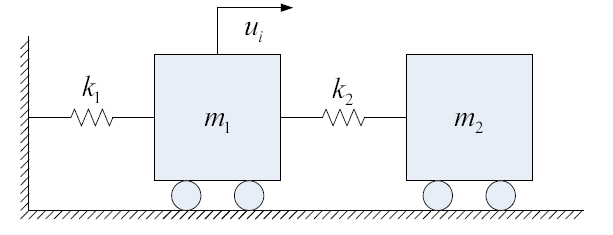
\includegraphics[scale=0.7]{images/excoop.png}
\end{figure}
\noindent
Each agent can be modeled as follows: 
\begin{equation*}
    \begin{aligned}
        &\dot{x}_i = A x_i + B u_i\\
        &y = Cx_i
    \end{aligned}
\end{equation*}

where $x_i = [p_1^i, \ v_1^i, \  p_2^i, \ v_2^i]^T$ where $p_1, p_2$ are the \textit{displacement} with respect to the position \textbf{at rest}. The input $u_i$ is a force applied to the mass $m_1$ of each agent $S_i$. The values for the parameters are: $m_1 = 1.1 \ kg$, $m_2 = 0.9 \ kg$, $K_1 = 1.5 \ N/m$, $K_2 = 1 \ N/m$. Note that \textbf{the leader node is unforced} that is $u_0=0$.

The multi-agent system is made up of a \textbf{leader node} and \textbf{six follower nodes} which are interconnected following the graph in the figure below

\begin{figure}[h]
    \centering
    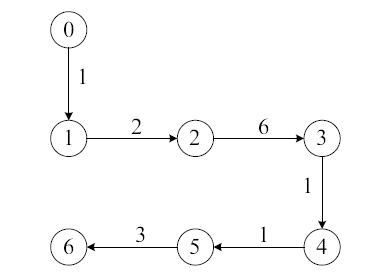
\includegraphics[scale=1]{images/graphTop.png}
\end{figure}

The objective here is to design a global cooperative tracking controller in order to follow the trajectory dictated by the leader node which is producing a desired trajectory. Let's assume randomly generated values for the initial conditions for all the state variables $x_i$.\\
As further step you can consider that the state is not fully measurable and to build a cooperative controller following the two proposed approaches  and then by using such an estimate to design a SVFB protocol. In other words the additive task is to design a \textit{cooperative distributed dynamic regulator}. In order to carry out this task you can assume (in a quite realistic way) that only positions are measurable, the resulting matrix $C$ to be used is the following: 
\begin{equation*}
    C = \begin{bmatrix}
        1&0&0&0\\
        0&0&1&0
    \end{bmatrix}
\end{equation*}





